\documentclass[UKenglish,usenames,dvipsnames,svgnames,table,aspectratio=169,mathserif]{beamer}

\mode<presentation> {

%\usetheme{default}
\usetheme{Madrid}

\setbeamertemplate{footline} % To remove the footer line in all slides uncomment this line

\setbeamertemplate{navigation symbols}{} % To remove the navigation symbols from the bottom of all slides uncomment this line
}

\usepackage{graphicx} % Allows including images
\usepackage{booktabs} % Allows the use of \toprule, \midrule and \bottomrule in tables
\usepackage{hyperref}
%\usepackage{apacite}
\usepackage{babel}
\usepackage{fancyvrb}
\usepackage{color}
\usepackage{alltt}
\usepackage{listings}
\usepackage{framed}
\usepackage{courier}
\usepackage{minted}
\usepackage{epstopdf}
\usepackage{xifthen}
\usepackage[utf8]{inputenc}
\usepackage[T1]{fontenc}
\usepackage{textcomp}
\usepackage{gensymb}
\usepackage{svg}
\usepackage{pdfpages}
\usepackage{isodate}
\usepackage{Haskelllogo}

\hypersetup{colorlinks=false}

\setbeamertemplate{bibliography entry title}{}
\setbeamertemplate{bibliography entry location}{}
\setbeamertemplate{bibliography entry note}{}
\setbeamertemplate{itemize items}[circle]
\setbeamertemplate{enumerate items}[circle]
\beamertemplatenavigationsymbolsempty
\setbeamertemplate{footline}{}


\newminted{haskell}{}

\definecolor{g}{RGB}{0,100,0}
\newcommand{\highlight}[1]{\colorbox{yellow}{#1}}
\newcommand{\nega}[1]{\colorbox{yellow}{#1}}
\newcommand{\posi}[1]{\colorbox{green}{#1}}
\newcommand{\nl}{\vspace{\baselineskip}}
\newcommand{\pnl}{\pause \nl}

\graphicspath{{diagrams/}}

\newcommand{\textslide}[1]{{
\begin{frame}
\begin{center}

#1

\end{center}
\end{frame}
}}

\newcommand{\textslideleft}[1]{{
\begin{frame}

#1

\end{frame}
}}

\newcommand{\codeslide}[1]{{
\begin{frame}[fragile]
\begin{haskellcode}
#1
\end{haskellcode}
\end{frame}
}}


\newcommand{\imageslide}[2][1]{{
\begin{frame}\begin{center}
\includegraphics[scale=#1]{#2}
\end{center}\end{frame}
}}

\newcommand{\imageslideleft}[2][1]{{
\begin{frame}
\includegraphics[scale=#1]{#2}
\end{frame}
}}

\newcommand{\imagetextslide}[3][1]{{
\begin{frame}\begin{center}

{#3}

\includegraphics[scale=#1]{#2}
\end{center}\end{frame}
}}

\newcommand{\svgslide}[1]{{
\begin{frame}
\begin{center}
\includesvg{diagrams/#1}
\end{center}
\end{frame}
}}

\newcommand{\latticeinfoslide}[1]{{
\begin{frame}
\begin{columns}
\column{0.7\textwidth}
\includegraphics[scale=0.65]{#1}
\column{0.3\textwidth}
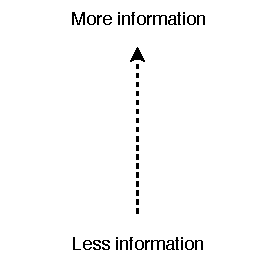
\includegraphics[scale=1.2]{set/more-info.pdf}
\end{columns}
\end{frame}
}}

\newcommand{\ctof}{{
\LARGE $\degree F = \degree C \times \frac{9}{5} + 32$
}}

\newcommand{\ftoc}{{
\LARGE $\degree C = (\degree F - 32) \div \frac{9}{5}$
}}

\definecolor{bgc}{RGB}{255, 255, 255}
\setbeamercolor{background canvas}{bg=bgc}

%%----------------------------------------------------------------------------------------
%	TITLE PAGE
%----------------------------------------------------------------------------------------

\title[Propagators]{An Intuition for Propagators}
\titlegraphic{
\includegraphics[scale=0.25]{data61.png}}
\author{George Wilson}
\institute[]
{
CSIRO's Data61\\
\medskip
\href{george.wilson@data61.csiro.au}{george.wilson@data61.csiro.au}
}

\selectlanguage{UKenglish}
\date{\printdate{2019-09-02}}

\begin{document}

%%%%%
%%%%% Intro section
%%%%%

\begin{frame}
\titlepage
\end{frame}


\begin{frame}

\huge \centering 1970s, MIT
\end{frame}


\begin{frame}

\Large \centering
a model of computation for {\bf highly parallel} machines
\end{frame}


\begin{frame}[fragile]

\begin{columns}
\begin{column}{0.5\textwidth}
\begin{overlayarea}{0.5\textwidth}{0.5\textheight}
\begin{onlyenv}<1>
\includegraphics[scale=1.3]{intro-cell0.pdf}
\end{onlyenv}
\begin{onlyenv}<2>
\includegraphics[scale=1.3]{intro-cell1.pdf}
\end{onlyenv}
\begin{onlyenv}<3>
\includegraphics[scale=1.3]{intro-cell2.pdf}
\end{onlyenv}
\end{overlayarea}
\end{column}
\begin{column}{0.5\textwidth}
\begin{overlayarea}{0.5\textwidth}{0.5\textheight}
\begin{onlyenv}<1->
\begin{haskellcode}
do
  c <- cell
\end{haskellcode}
\end{onlyenv}
\begin{onlyenv}<2->
\begin{haskellcode}
  write c "Hello"
\end{haskellcode}
\end{onlyenv}
\begin{onlyenv}<3->
\begin{haskellcode}
  write c "Compose"
\end{haskellcode}
\end{onlyenv}
\end{overlayarea}
\end{column}
\end{columns}
\end{frame}


\begin{frame}[fragile]
\centering

\begin{columns}
\begin{column}{0.5\textwidth}
\begin{overlayarea}{0.5\textwidth}{0.4\textheight}
\begin{onlyenv}<1>
\includegraphics[scale=0.8]{intro-toUpper1.pdf}
\end{onlyenv}
\begin{onlyenv}<2>
\includegraphics[scale=0.8]{intro-toUpper2.pdf}
\end{onlyenv}
\begin{onlyenv}<3>
\includegraphics[scale=0.8]{intro-toUpper3.pdf}
\end{onlyenv}
\begin{onlyenv}<4->
\includegraphics[scale=0.8]{intro-toUpper4.pdf}
\end{onlyenv}
\end{overlayarea}
\end{column}

\begin{column}{0.5\textwidth}
\begin{overlayarea}{\textwidth}{0.3\textheight}
\begin{onlyenv}<1->
\begin{haskellcode}
do
  input  <- cell
\end{haskellcode}
\begin{haskellcode}
  output <- cell
\end{haskellcode}
\end{onlyenv}
\begin{onlyenv}<2->
\begin{haskellcode}
  lift toUpper input output
\end{haskellcode}
\end{onlyenv}
\end{overlayarea}
\begin{overlayarea}{\textwidth}{0.2\textheight}
\begin{onlyenv}<3->
\begin{haskellcode}
  -- run the network
  write input 'q'
\end{haskellcode}
\end{onlyenv}
\begin{onlyenv}<5->
\begin{haskellcode}
  content output   -- Just 'Q'
\end{haskellcode}
\end{onlyenv}
\end{overlayarea}
\end{column}
\end{columns}
\end{frame}


\begin{frame}[fragile]
\centering

\begin{columns}
\begin{column}{0.5\textwidth}
\nl
\begin{overlayarea}{0.5\textwidth}{0.4\textheight}
\begin{onlyenv}<1>
\includegraphics[scale=0.9]{build-bidirectional-adder0.pdf}
\end{onlyenv}
\begin{onlyenv}<2>
\includegraphics[scale=0.9]{build-bidirectional-adder1.pdf}
\end{onlyenv}
\end{overlayarea}
\end{column}

\begin{column}{0.5\textwidth}
\begin{overlayarea}{0.5\textwidth}{0.3\textheight}
\begin{onlyenv}<1->
\begin{haskellcode}
do
  inL  <- cell
  inR  <- cell
  out  <- cell
\end{haskellcode}
\end{onlyenv}
\nl
\begin{onlyenv}<2->
\begin{haskellcode}
  adder inL inR out
\end{haskellcode}
\end{onlyenv}
\end{overlayarea}

\begin{overlayarea}{0.5\textwidth}{0.3\textheight}
\invisible{phantom}
\begin{onlyenv}<2>
\begin{haskellcode}
    where
      adder l r o = do
        lift2 (+) l r o
\end{haskellcode}
\end{onlyenv}
\end{overlayarea}
\end{column}

\end{columns}
\end{frame}


\begin{frame}

\begin{center}
\begin{LARGE}
\begin{overlayarea}{0.2\textwidth}{0.5\textheight}
\begin{onlyenv}<1>
$z =\ x + y$
\end{onlyenv}
\begin{onlyenv}<2>
$z \leftarrow x + y$
\end{onlyenv}
\begin{onlyenv}<3>
$z \leftarrow x + y$ \\
$x \leftarrow z - y$ \\
$y \leftarrow z - x$ \\
\end{onlyenv}
\end{overlayarea}
\end{LARGE}
\end{center}
\end{frame}


\begin{frame}[fragile]
\centering

\begin{columns}
\begin{column}{0.5\textwidth}
\nl
\begin{overlayarea}{0.5\textwidth}{0.4\textheight}
\includegraphics[scale=0.9]{build-bidirectional-adder2.pdf}
\end{overlayarea}
\end{column}

\begin{column}{0.5\textwidth}
\begin{overlayarea}{0.5\textwidth}{0.3\textheight}
\begin{haskellcode}
do
  inL  <- cell
  inR  <- cell
  out  <- cell
\end{haskellcode}
\nl
\begin{haskellcode}
  adder inL inR out
\end{haskellcode}
\end{overlayarea}

\begin{overlayarea}{0.5\textwidth}{0.3\textheight}
\invisible{phantom}
\begin{haskellcode}
    where
      adder l r o = do
        lift2 (+) l r o
        lift2 (-) o l r
        lift2 (-) o r l
\end{haskellcode}
\end{overlayarea}
\end{column}

\end{columns}
\end{frame}


\imagetextslide[0.8]{celsius/celsius5.pdf}{\ctof \\ \nl \ftoc}
\imagetextslide[0.8]{celsius/celsius6.pdf}{\ctof \\ \nl \ftoc}
\imagetextslide[0.8]{celsius/celsius7.pdf}{\ctof \\ \nl \ftoc}
\imagetextslide[0.8]{celsius/celsius8.pdf}{\ctof \\ \nl \ftoc}


\imageslide{oscillator0.pdf}
\imageslide{oscillator1.pdf}
\imageslide{oscillator2.pdf}
\imageslide{oscillator3.pdf}
\imageslide{oscillator4.pdf}
\imageslide{oscillator5.pdf}
\imageslide{oscillator6.pdf}
\imageslide{oscillator7.pdf}
\imageslide{oscillator8.pdf}


\begin{frame}
\centering
\fontsize{60}{70}\selectfont $?!$

\end{frame}


\begin{frame}
\centering \huge

How can we fix this?
\end{frame}


\begin{frame}[fragile]
\begin{columns}
\column{0.1\textwidth}
\column{0.7\textwidth}
\begin{overlayarea}{\textwidth}{0.6\textheight}
\begin{haskellcode}
data WriteOnce a
  = None
  | Written a
  | TooMany
\end{haskellcode}

\nl

\begin{onlyenv}<2>
\begin{haskellcode}
tryWrite ::           a -> WriteOnce a -> WriteOnce a
tryWrite a w = case w of
  None      -> Written a
  Written b -> TooMany
  TooMany   -> TooMany
\end{haskellcode}
\end{onlyenv}

\begin{onlyenv}<3->
\begin{haskellcode}
tryWrite :: (Eq a) => a -> WriteOnce a -> WriteOnce a
tryWrite a w = case w of
  None      -> Written a
  Written b -> if a == b then Written b else TooMany
  TooMany   -> TooMany
\end{haskellcode}
\end{onlyenv}
\end{overlayarea}
\column{0.2\textwidth}
\end{columns}
\end{frame}


\imageslide{oscillator-fixed1.pdf}
\imageslide{oscillator-fixed2.pdf}
\imageslide{oscillator-fixed3.pdf}
\imageslide{oscillator-fixed4.pdf}
\imageslide{oscillator-fixed5.pdf}
\imageslide{oscillator-fixed6.pdf}
\imageslide{oscillator-fixed7.pdf}


\begin{frame}

\centering \LARGE

Mutability is {\bf chaos}

\nl
WriteOnce is {\bf rigid}
\end{frame}


\begin{frame}[fragile]

\LARGE
\begin{center}
Accumulate information about a value

% \pnl

% {\bf monotonically}
\end{center}
\end{frame}


% \begin{frame}

% \centering \huge
% Monotonicity
% \nl

% \Large
% $f$ is monotone if\\
% \nl

% $ x \leq y \implies f(x) \leq f(y)$

% \end{frame}


% \begin{frame}
% \Large

% Now every network will give a
% {\bf deterministic answer}
% in {\bf finite time}
% \end{frame}


\begin{frame}[fragile]

\begin{columns}

\begin{column}{0.3\textwidth}
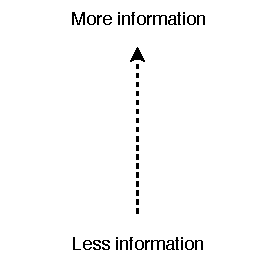
\includegraphics[scale=1.3]{set/more-info.pdf}
\end{column}

\begin{column}{0.6\textwidth}
\begin{haskellcode}
  -- I have heard contradictory answers!
    TooMany

  -- I know the answer exactly
    Written a

  -- I don't know anything
    None
\end{haskellcode}

\end{column}

\end{columns}
\end{frame}


\imageslide[0.6]{sudoku/sudoku1.png}
\imageslide[0.6]{sudoku/sudoku2.png}
\imageslide[0.6]{sudoku/sudoku3.png}
\imageslide[0.6]{sudoku/sudoku4.png}
\imageslide[0.6]{sudoku/sudoku5.png}
\imageslide[0.6]{sudoku/sudoku6.png}
\imageslide[0.6]{sudoku/sudoku7.png}
\imageslide[0.6]{sudoku/sudoku8.png}
\imageslide[0.6]{sudoku/sudoku9.png}
\imageslide[0.6]{sudoku/sudoku10.png}
\imageslide[0.6]{sudoku/sudoku11.png}
\imageslide[0.6]{sudoku/sudoku12.png}
\imageslide[0.6]{sudoku/sudoku13.png}


\begin{frame}
\begin{columns}
\column{0.7\textwidth}
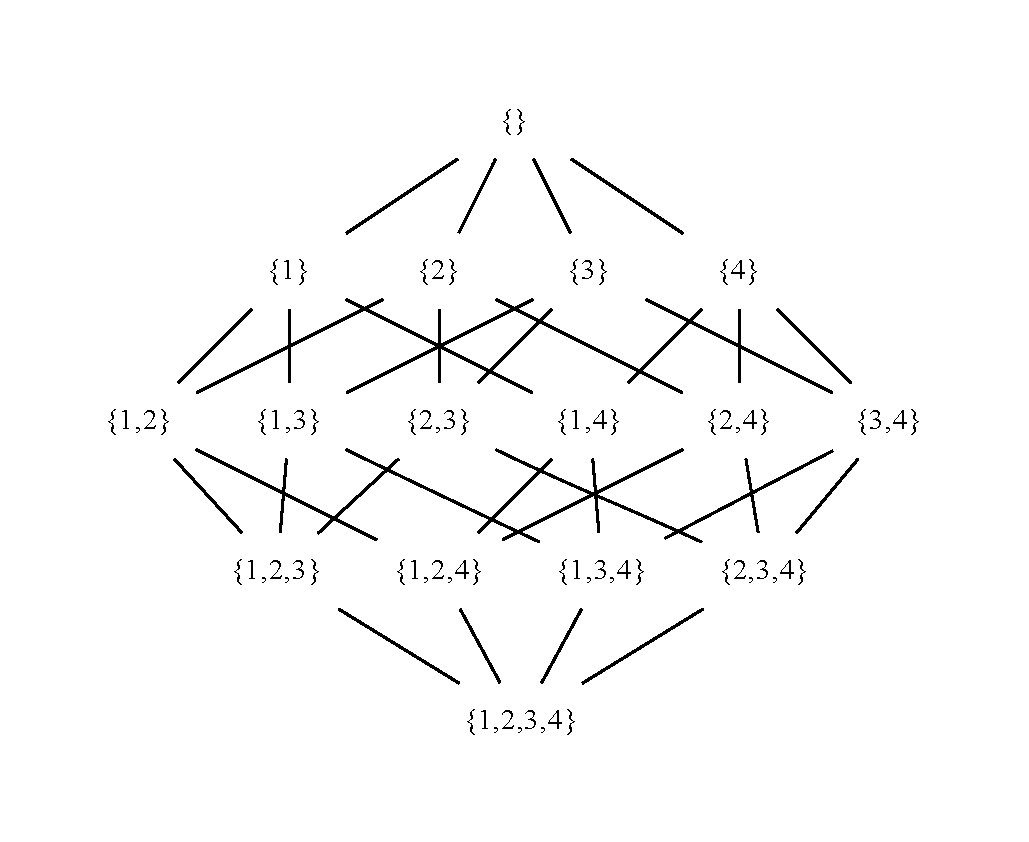
\includegraphics[scale=0.65]{set/powerset.pdf}
\pause
\column{0.3\textwidth}
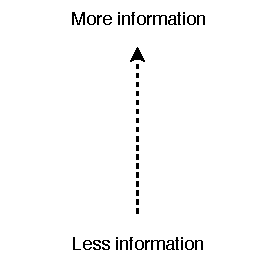
\includegraphics[scale=1.2]{set/more-info.pdf}
\end{columns}
\end{frame}


\latticeinfoslide{set/powerset-info1.pdf}
\latticeinfoslide{set/powerset-info2.pdf}
\latticeinfoslide{set/powerset-info3.pdf}
\latticeinfoslide{set/powerset-info4.pdf}

\latticeinfoslide{set/powerset1.pdf}
\latticeinfoslide{set/powerset2.pdf}
\latticeinfoslide{set/powerset3.pdf}
\latticeinfoslide{set/powerset4.pdf}
\latticeinfoslide{set/powerset5.pdf}
\latticeinfoslide{set/powerset6.pdf}


% \begin{frame}

% The accumulation must:

% \begin{itemize}
% \item tolerate {\bf reordering} of information
% \item tolerate {\bf grouping} of information
% \item ignore {\bf redundancy} of information
% \end{itemize}
% \end{frame}

% \begin{frame}

% To be deterministic we must

% \begin{itemize}
% \item tolerate {\bf reordering} of writes
% \item tolerate {\bf grouping} of writes
% \item ignore {\bf redundancy} of writes
% \end{itemize}
% \end{frame}


\begin{frame}[fragile]
\centering \huge
Bounded join semilattice
\nl
\large

Identity: \\
$x \vee bottom = bottom = bottom \vee x$
\nl

Associative: \\
$x \vee (y \vee z) = (x \vee y) \vee z$
\nl

Commutative: \\
$x \vee y = y \vee x$
\nl

Idempotent: \\
$x \vee x = x$

\end{frame}


\begin{frame}[fragile]

\begin{overlayarea}{\textwidth}{0.5\textheight}
\begin{haskellcode}
class SemiLattice a where
  (\/)   :: a -> a -> a
  bottom :: a
\end{haskellcode}
\nl

\begin{onlyenv}<2-3>
\begin{haskellcode}
data SudokuVal = One | Two | Three | Four
  deriving (Eq, Ord)

data Possibilities = P (Set SudokuVal)
\end{haskellcode}
\end{onlyenv}
\nl
\begin{onlyenv}<3>
\begin{haskellcode}
instance Semilattice Possibilities where
  P p \/ P q = P (Set.intersection p q)
  bottom = P (Set.fromList [One,Two,Three,Four])
\end{haskellcode}
\end{onlyenv}
% \begin{onlyenv}<4>
% \begin{haskellcode}
% instance (Eq a) => SemiLattice (WriteOnce a) where
%   None      \/ b           = b
%   TooMany   \/ x           = TooMany
%   Written a \/ None        = Written a
%   Written a \/ TooMany     = TooMany
%   Written a \/ Written b   = if a == b then Written a else TooMany
% \end{haskellcode}
% \end{onlyenv}
\end{overlayarea}
\end{frame}


\begin{frame}
\begin{columns}
\column{0.7\textwidth}
\includegraphics{writeonce-bool0.pdf}
\column{0.3\textwidth}
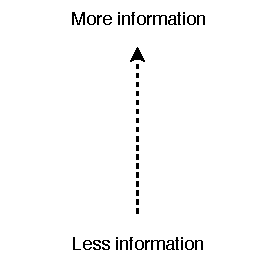
\includegraphics[scale=1.3]{set/more-info.pdf}
\end{columns}
\end{frame}


\begin{frame}
\LARGE \centering

Cells hold semilattices

Propagators join information in
\end{frame}


\begin{frame}

\centering
WriteOnce \\
Sets (intersection or union) \\
Intervals \\
Search \\
Unification \\
many more
\end{frame}


\begin{frame}
\huge \centering
Thanks for listening!
\nl

\large
Working code for all these examples and more:

\url{https://github.com/qfpl/propagator-examples}

\end{frame}

\begin{frame}

{\Large \bf
References}

Art of the propagator: \\
\url{https://dspace.mit.edu/handle/1721.1/44215}

Alexey Radul's PhD Thesis: \\
\url{https://dspace.mit.edu/handle/1721.1/54635}

Edward Kmett at Boston Haskell: \\
\url{https://www.youtube.com/watch?v=DyPzPeOPgUE}

George Wilson on semi-lattices: \\
\url{https://www.youtube.com/watch?v=VXl0EEd8IcU}

\nl
{\Large \bf
Implementations}

Fancy experimental implementation: \\
\url{https://github.com/ekmett/guanxi}

Propagators in Haskell \\
\url{https://github.com/ekmett/propagators}

Propagators in Clojure: \\
\url{https://github.com/tgk/propaganda}

\end{frame}


\end{document}
